% !TEX root = ../thesis.tex
%
\chapter{System Design}
\label{ch:design}

After consideration of the goals for the \acf{IFAS} and the results from the classifications made earlier (cf. \cref{ch:classifications}), the system was designed.
This activity includes specific decisions such as which data to collect and especially how to implement the Event Store-Elasticsearch bridge service, as well as working out the overall architecture of the whole system.

\section{Metrics Selection}
\label{sec:design:metrics}

WIP
\cite{Kelly:2003:IFI:959258.959260}
\cite{Claypool2001} % Scrolling vs. explicit rating: good indicator
\cite{Claypool2001} % Time spent on page vs explicit rating: good indicator

% Identifying the metrics to evaluate created customer value and product success was a challenge both in relation to dedicated experiments and to the general observation of product usage \cite{lindgren2015software}

% active channel usage (posted msgs)
% passive channel usage (scrolling)
% clicking (?)


\section{User Feedback Events}
\label{sec:design:event-structure}

User feedback is sent to \ac{IFAS} in the form of events, as the data is internally first saved in \ac{IFAS}' Event Store.
All events are saved to a single Event Store stream; this helps to isolate the user feedback data separated from other data that may be posted to Event Store in a production environment.

In order to supply the data that is necessary for the metrics defined earlier, five different event types were created.
These event types are listed below, together with a description of the data that they provide and in which cases they are sent to \ac{IFAS}:

\begin{description}
\item[ChannelSwitched]
Whenever a user switches the messaging channel, this event is sent.
It contains data about the channel that is switched to, as well as the method of channel switching: Via the left-side menu bar, or via the \emph{channel switcher} feature.
\item[TutorialExperimentParticipated]
This event contains information about the decision a newly registered user makes regarding the Mattermost tutorial:
Either the user participates in the tutorial, or they skip it.
As this event is used as the data source for an A/B test, it also contains information about the group that the user was assigned to, which is either control or treatment.
\item[PostCreated]
Every time a message is sent in Mattermost, a new \texttt{PostCreated} event is fired.
This event contains extensive data about the message itself, such as its contents and the sender's id, as well as a lot of metadata such as the channel the message was posted to and the time it was created.
The resulting data is used to compute the metric regarding active channel usage.
\item[UserClicked]
These events are used to capture all clicks that a user performs in the application.
The intention is that for any application, these events give an analyst enough information to identify what the user was doing at any given point.
The \texttt{UserClicked} event contains information about the clicked element such as the HTML attributes \texttt{class} and \texttt{id} as well as its inner text.
There may still be cases where this is not enough to identify the action that the user performed, which is why the event is amended with the click's position within the application, the window's height and width, and the current URL.
Using this information, the analyst can exactly identify the position where the user clicked at the given point in time.
\item[WindowScrolled]
Whenever a user scrolls up or down in the chat window, a \texttt{WindowScrolled} event is sent to \ac{IFAS}.
This event encaspulates information about the URL at which the scrolling occured, as well as the duration and amount of the scrolling.
Using this event's data, the scrolling amount metric can be computed.
\end{description}

Parts of the data contained in these events may be redundant or unspecific in some cases, but helps to recreate the user's steps if this is needed.
The additional data could also be used to later measure additional metrics.
%If this is undesirable because the additional data takes up too much disk space, or because of moral concerns regarding the hoarding 
In a production environment, the specificity of these events could be improved by assigning unique ids to every element in the web application, or at least to the ones which are of special interest.
Especially the \texttt{UserClicked} events would benefit from this.

\section{Event Store-Elasticsearch Bridge}
\label{sec:design:bridge}

In order to move the event data to Elasticsearch and afterwards into Kibana, a service is needed which bypasses the lack of a direct integration of Event Store and Elasticsearch.
This service is the Event Store-Elasticsearch bridge (short just ``bridge'' in this context).

%\subsection{The Need for a Bridge Service}

Intuitively, it seems problematic that Event Store and Elasticsearch have different concepts of storing their data.
On the one hand, Event Store data is stored as events in streams; each event always has an event type and a unique id within that stream.
On the other hand, in Elasticsearch, data is managed in indices which contain documents; each Elasticsearch document is assigned a document type.

The bridge spans the gap between the two concepts by subscribing to all events that are posted to the user feedback stream and posting them to Elasticsearch.
As Elasticsearch does not allow multiple document types in the same index since the release of the most recent major version\footnote{\url{https://www.elastic.co/guide/en/elasticsearch/reference/current/removal-of-types.html}}, each event type has to have its own Elasticsearch index.
Thus, \ac{IFAS} in its current state has five Elasticsearch indices, one for each event type.
The index names always have the Event Store stream's name as the prefix and the event type as the suffix, divided by an underscore.
In conclusion, each stream maps to the prefix of an index, each event type maps to the suffix of an index, and each event maps to a document (cf. \cref{table:design:bridge}).
The event type is automatically also the document type.

%This is also benefical for later analysis in Kibana, as indices with multiple document types would clutter the \ac{UI}

\begin{table}[ht]
\centering
\caption{Mapping of Event Store to Elasticsearch data types.}
\label{table:design:bridge}
\begin{tabular}{l|l}
\textbf{Event Store} & \textbf{Elasticsearch} \\ \cline{1-2}
Stream & Index prefix \\
Event type & Index suffix \& document type \\
Event & Document
\end{tabular}
\end{table}

One possible and seemingly convenient solution would be using Logstash\footnote{\url{https://www.elastic.co/products/logstash}} as the bridge, which is not applicable in this exact scenario though.
Logstash is another application from the Elastic stack; it serves the exact purpose to integrate data from various sources into Elasticsearch.
It is possible to consume Atom feeds via Logstash's \ac{RSS} plugin, which Event Store offers an interface for.
This is not feasible in this scenario as Logstash's \ac{RSS} plugin is not able to handle feeds which require authentication, which Event Store does.
Also, Event Store's persistent subscriptions are not compatible with Atom feeds, which is another reason to abandon Logstash as a possible solution.

Instead of using an existing service that listens to Atom feeds such as Logstash, a custom implementation is the better approach here.
This is the case because the official .NET Core Event Store client \ac{API}\footnote{\url{https://github.com/EventStore/ClientAPI.NetCore}} can be used, which allows amongst others for usage of persistent subscriptions and more efficient communication over a dedicated protocol built on top of \ac{TCP}.
The \ac{TCP} protocol variant is faster than the alternative via Atom feeds, which is built on top of \ac{HTTP}~\cite{WEB:EvtSt-Which-Api}.
It should be noted that, although using \ac{TCP} instead of \ac{HTTP} contradicts the requirement for an \ac{HTTP} interface as stated in \cref{sec:design:goals}, this is not a problem at all due to the heterogenous technology that a microservice architecture allows~\cite[Key Benefits,pp.~4f]{newman2015building}.

Assuming the Event Store stream already exists, setting up the bridge to transfer new events to an Elasticsearch index would then be a two-step process.
First, a persistent subscription has to be created within the Event Store administration overlay.
Then, an instance of the bridge service has to be started, configured to listen to the newly created subscription.
This would cause the bridge to transfer all existing events which were not read previously to the respective Elasticsearch indices, and then also posting all subsequently received events to this index.

It would also be possible to implement the bridge in a way that allows the service to listen to multiple subscriptions simultaneously.
This would require a more complex service which introduces two problems.
First, it introduces an unnecessary implementation overhead, and second, its additional complexity could lead to scaling problems.
Writing complex, large serices is in general discouraged to do in a microservice architecture~\cite[Key Benefits,pp.~5f]{newman2015building}.
Instead, multiple instances of the same service should be executed alongside each other, with their respective configuration for listening to a specific stream.

Thanks to persistent subscriptions, it is possible to temporarily take the bridge instance offline -- as the subscription state is persisted on the server side, the bridge can transfer all events that occurred while it was offline as soon as it comes online again.
Multiple instances of the bridge may listen to the same persistent subscription if heavy load is expected on the system -- this is known as the \emph{competing consumers} messaging pattern~\cite{WEB:Microsoft-Competing-Consumers}.
This advanced use case is not considered further though.

When a persistent subscription is created -- which the bridge assumes has already happened -- it expects a stream name and a \emph{subscription group} as parameters.
There can be multiple persistent subscriptions of different groups listening to the same stream; the subscriptions then operate independently of each other.
This pattern is rather useful if the data from a given stream is used by another application alongside \ac{IFAS}.

%\subsection{Mapping Event Store Rebuilds to Elasticsearch}
%\label{subsec:design:bridge:mapping}

Another advanced feature of Event Store are the complete rebuild, event replay and reversing of events.
This is supported indirectly in \ac{IFAS} by first deleting the appropriate documents from the respective Elasticsearch index, which can be done using the Delete By Query API\footnote{\url{https://www.elastic.co/guide/en/elasticsearch/reference/current/docs-delete-by-query.html}}.
In the case of a complete rebuild, the index can be completely emptied.
Then, when the rebuild, replay or reversing is executed in Event Store, the persistent subscription can forward all rebuilt events to the bridge.
The downside is that this introduces a delay in which the analytics application is practically useless, depending on the complexity and amount of events this can be an important factor.
\todo{Test this or trow it out!}

\section{Final Architecture}
\label{section:design:architecture}

Each \ac{IFAS} component is implemented as a standalone Docker container that communicates with the other services via \ac{TCP} or \ac{HTTP}.
These containers are executed in one multi-container Docker application, whose architecture is visualized in \cref{figure:design:architecture}.

The services that implement the main functionality of \ac{IFAS} are the three integral services discussed in \cref{ch:classifications} -- data storage, aggregation, and analysis -- as well as the bridge between storage and aggregation.
The bridge connects to the Event Store container via its port 1113 over \ac{TCP}, and to Elasticsearch via port 9200 over \ac{HTTP}.
Kibana also communicates with Elasticsearch over the same port.
All this communication occurs exclusively over the internal network of the \ac{IFAS} Docker application, but two ports are exposed such that the system can properly be interacted with.
These are Event Store's port 2113 -- i.e. the \ac{HTTP} interface -- in order to allow the client application to send data to \ac{IFAS}, and Kibana's port 5601 which exposes the Kibana application for usage via a web browser.

This Docker application also includes the services running the Mattermost client.
The diagram displays an abstraction of the client component, which internally consists of three services:
The Mattermost server, the customized Mattermost web application, and an Nginx service which exposes the web application for usage via a web browser to port 80.
As \ac{IFAS} is agnostic of the client application that serves the user feedback, this is merely displayed as ``Mattermost'' in the diagram.
Details about this setup go beyond the scope of this thesis, but can be read up on the Github page for the Mattermost-Docker repository\footnote{\url{https://github.com/mattermost/mattermost-docker}}.
Data is transfered to \ac{IFAS} via its exposed port 2113, which the Mattermost web application connects to.
It would also be possible to run the client application in a separate environment; the only required change would be to expose port 2113 of the Event Store container such that the client can send events from outside the Docker application.

\begin{figure}[ht]
\makebox[\textwidth][c]{
        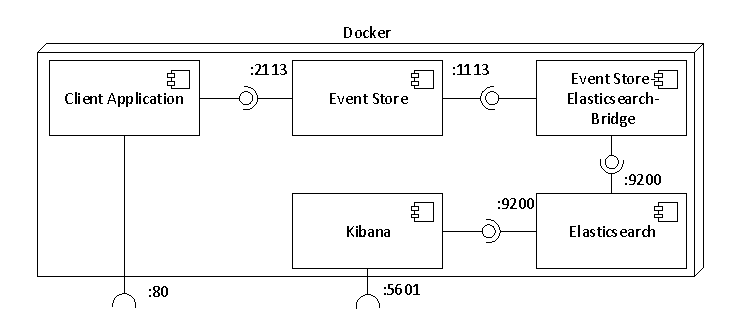
\includegraphics[width=1.2\textwidth]{gfx/docker-architecture.pdf}
}
        \caption{Structure diagram of the final architecture of \ac{IFAS}.}
        \label{figure:design:architecture}
\end{figure}
